% FIX:
\documentclass[tikz,border=4]{standalone}
\usetikzlibrary{decorations}

\pgfkeys{/pgf/decoration/.cd,
  stipple density/.store in=\pgfstippledensity,
  stipple density=(sin(\pgfstipplex*180)*0.25+0.1),
  stipple amplitude/.store in=\pgfstippleamplitude,
  stipple amplitude=(rnd^3)*\pgfstippley*(sin(\pgfstipplex*180)^2+0.05),
  % stipple scaling function/.store in=\pgfstipplescalingfunction,
  % stipple scaling function=sin(\pgfstipplex*180)*0.875+0.125,
  stipple radius/.store in=\pgfstippleradius,
  stipple radius=0.25pt
}

\pgfdeclaredecoration{stipple}{draw}{
\state{draw}[width=\pgfdecorationsegmentlength]{%
  \pgfmathparse{\pgfdecoratedcompleteddistance/\pgfdecoratedpathlength}%
  \let\pgfstipplex=\pgfmathresult%
  \let\pgfstippley=\pgfdecorationsegmentamplitude%
  \pgfmathparse{int(abs((\pgfstippledensity)*100))}%
  \let\pgfstipplen=\pgfmathresult%
  \pgfmathloop%
  \ifnum\pgfmathcounter<\pgfmathresult\relax%
    \pgfpathcircle{%
      \pgfpoint{(rnd-0.5)*\pgfdecorationsegmentlength}%
        % {(\pgfstipplescalingfunction)*(rnd^4)*\pgfdecorationsegmentamplitude+\pgfstippleradius}}%
        {(\pgfstippleamplitude)+\pgfstippleradius}}%
    {\pgfstippleradius}%
  \repeatpgfmathloop%
}
}

\tikzset{stipple/.style={
  decoration={stipple, segment length=2pt, #1},
  decorate,
  fill
}}

\begin{document}
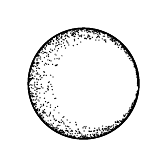
\begin{tikzpicture}[x=2em,y=2em]
	% Layer 1: Outer ring (full density)
	\draw [postaction={stipple={amplitude=0.3cm, stipple density=.15}}]
	(0,0) circle [radius=1];
	% Layer 2: Middle ring (reduced density)
	\draw [postaction={stipple={amplitude=0.2cm, stipple density=.08}}]
	(0,0) circle [radius=1];
	% Layer 3: Inner area (even more reduced)
	\draw [postaction={stipple={amplitude=0.1cm, stipple density=.03}}]
	(0,0) circle [radius=1];
\end{tikzpicture}

\begin{tikzpicture}[x=2em,y=2em]
	\draw [postaction={stipple={amplitude=0.5cm}},
		postaction={stipple={amplitude=0.25cm}}]
	(2,1) ..controls ++(135:1) and ++(90:1) ..
	(0,0) .. controls ++(270:1) and ++(180:1.5) ..
	(2,-2) .. controls ++(0:1.5) and ++(270:2) .. (5/2,0);
	% \draw [postaction={stipple={amplitude=0.5cm}},
	% 	postaction={stipple={amplitude=0.25cm}}]
	% (2,1) ..controls ++(135:1) and ++(90:1) ..
	% (0,0) .. controls ++(270:1) and ++(180:1.5) ..
	% (2,-2) .. controls ++(0:1.5) and ++(270:2) ..
	% (5,1) .. controls ++(90:2) and ++(75:1) ..
	% (2,1) .. controls ++(255:1/4) and ++(0:1/2) .. (3/2,0);
	\draw [postaction={stipple={amplitude=0.125cm, stipple density=0.05}},
		postaction={stipple={amplitude=0.5cm, reverse path}},
		postaction={stipple={amplitude=0.25cm, reverse path}}]
	(3,0) .. controls ++(135:1) and ++(90:1) .. (4,1);
\end{tikzpicture}
\end{document}
